\documentclass[12pt]{article}
\usepackage[margin=1in]{geometry}

\usepackage{wrapfig}
\usepackage{graphicx}
\graphicspath{ {figures/} }

\usepackage{enumerate}
\usepackage{enumitem}
\setlist{nolistsep}

\usepackage[numbers]{natbib}


\title{Understanding the Clinical Microbiome \\ Biological Engineering Thesis Proposal}

\author{Claire Duvallet}
\date{October 11, 2016}

\begin{document}


\maketitle
\newpage
\tableofcontents

\begin{abstract}
Researchers and clinicians have long appreciated the contribution of microbes
to human disease. Recently, many studies have moved from analyzing the effect of
individual microbes on human health to studying the complex interactions between
microbial communities and their human hosts, due in large part to developments
in high throughput DNA sequencing. We are beginning to understand
that microbial communities are involved in disease and are also
integral to human health,
but there remains no clear understanding on the precise relationships between human 
microbial communities and disease. Certain microbial communities, like those
of the aerodigestive tract, remain drastically under-studied. On the other hand,
the gut microbiome is extensively studied but lacks
a synthesized understanding of the relationship between alterations in its
microbes to disease in general and to specific diseases.
This thesis will expand our understanding of the clinical relevance
of the human microbiome by characterizing the 
understudied aerodigestive tract microbiome,
synthesizing results from gut microbiome case-control studies across
all studied disease states, and developing a tool to enable generalizable analysis
of microbial communities. This work will identify promising candidates and approaches
for follow-up mechanistic studies, and will move the field toward a more
translationally-relevant understanding of the relationship between our microbes
and our health.



\end{abstract}
\newpage

\section{Overall objectives and specific aims}
\subsection{Overall objectives}
In spite of the recent increase in research on the human 
microbiome, there is not a clear consensus on the relationship between 
human microbial communities and disease. Microbes colonize our entire bodies,
supplementing our own functions, priming and training our immune 
systems, providing resistance to colonization 
by pathogens, and contributing to maintenance of health or progression of disease (REF). 
However, our knowledge of the human microbiome is imbalanced: some
body sites are much more extensively studied than others. 
Additionally, even the most extensively studied body sites lack a 
synthesized understanding of the clinical relevance of all studied human-microbe associations. 
Finally, translating microbial associations into biological hypotheses
remains challenging due to the lack of centralized tools and databases
for assigning biological meaning to groups of microbes.

This thesis will expand our understanding of the clinical microbiome in three ways.
First, I will characterize the relationships between the microbial communities
of the aerodigestive tract and their associations with clinical factors, 
increasing our basic understanding of this under-studied system.
Next, I will perform a meta-analysis of published case-control gut microbiome studies
across many disease states, synthesizing the extensive existing studies by 
identifying consistent microbial markers of health and disease.
Finally, I will curate groups of biologically related microbes
to enable enrichment analyses and generalizable interpretations
of results from microbiome studies. 

\subsection{Specific Aims}
\begin{description}
	\item[Aim 1] Apply standard methods to identify microbial 
	community characteristics associated with gastro-esophogeal reflux 
	disease and aspiration.
	\begin{enumerate}
		\item Quantify how lung, gastric, and throat microbial 
		communities are related.
		\item Identify clinical modulators of lung, gastric, and 
		throat microbial communities.
	\end{enumerate}
	\item[Aim 2] Perform a meta-analysis of case-control gut 
	microbiome studies to identify consistent microbial signatures 
	within and across multiple diseases.
	\begin{enumerate}
		\item Compile and process publicly available case-control gut 
		microbiome studies with a standardized method.
		\item Determine whether certain microbes are consistently 
		associated disease in general or with specific diseases.
		\item Identify relationships between physiologically-related 
		diseases by comparing their microbial characteristics.
	\end{enumerate}
	\item[Aim 3] Enable generalizable interpretations of microbiome 
	analyses by assigning bacteria to groups with similar functions 
	and known associations with disease.
	\begin{enumerate}
		\item Combine existing databases with targeted literature searches 
		to define \textit{microbe sets} based on known biological 
		relationships.
		\item Use machine-learning techniques to extract disease-
		associated \textit{microbe sets} from datasets collected in Aim 2.
		\item Develop these \textit{microbe sets} into a collaborative 
		tool for use in interpreting new microbiome studies.
	\end{enumerate}
\end{description}
\newpage

\section{Background and significance}
\textit{Three to five pages}

The topics addressed in this thesis are broad, but are all connected by
the motivation to better understand
clinically-relevant associations between microbes and their human hosts.
My work will focus on the microbial communities of two major body systems:
the aerodigestive and gastrointestinal tracts. To study these, I will 
use a combination of traditional analytical techniques, supplemented by 
novel methods as required. This section will provide background on
the aerodigestive tract, the gut microbiome, and analytical techniques 
used in microbiome studies. 

\subsection{Aerodigestive tract}

\subsubsection{Physiology and disease}
From an engineering perspective, the aerodigestive tract,
consisting of the upper gastrointestinal and respiratory tracts,
can be thought of as different compartments connected by the esophagus and windpipe (REF, FIGURE).
The mass transport between the throat, stomach, and lung compartments is regulated by complex physiological 
mechanisms. Swallowing guides material from the mouth to the stomach, 
but may dysfunction and allow material to enter the lungs. The 
esophageal sphincter usually prevents material from leaving the 
stomach, but in some diseases is dysfunctional. Finally, complex 
homeostatic mechanisms clear the lungs of foreign bodies and create a 
very selective environment for microbes in the lungs (REFS REFS REFS). 
Thus, while the throat, stomach, and lung "compartments" are 
physically connected, the amount of material, including bacteria, 
flowing between them is not readily apparent. 

Gastro-esophogeal reflux disease (GERD) is set of syndromes in which 
the reflux of stomach contents leads to troublesome symptoms or 
complications \cite{vakil-gerd_defn-2006},\cite{dent-gerd_epi-2005}
(FIGURE - Figure 2 of Vakil et al). The most common symptoms of GERD 
are regurgitation and heartburn, but the disease may also present 
asymptomatically\cite{vakil-gerd_defn-2006},\cite{dent-gerd_epi-2005}. 
GERD can be diagnosed by demonstrating reflux of gastric contents (via 
pH and impedance monitoring), injury to the esophogus (via endoscopy), 
or based on symptoms alone\cite{vakil-gerd_defn-2006}. GERD affects
A LOT OF PEOPLE and can lead to severe complications such as Barrett's 
esophagus (REF). Proton-pump inhibitors (PPIs) are often prescribed for GERD,
though long-term adverse effects of these drugs is becoming more widely understood (REFS - the PPI microbiome ref).
In cases of severe reflux, fundoplication surgery may
be recommended, in which part of the stomach is wrapped around the 
esophagus to prevent refluxate from leaving the stomach and going up
into the esophagus (REF). 

Aspiration is another complex aerodigestive condition which may result
from dysfunctional swallowing or through other mechanisms, the etiology and consequences of which are unclear.
Clinically, aspiration is defined as the inhalation of foreign material such as food or 
gastric contents into the lungs \cite{raghavendran-asp_injury-2011}. 
Most aspiration events are unwitnessed without obvious outward signs 
or symptoms, and may involved large quantities of aspirated material 
or may be micro-aspiration events \cite{raghavendran-asp_injury-2011}. 
Aspiration resulting from swallowing dysfunction can be diagnosed with 
a Modified Barium Swallow test (MBS) \cite{martinharris-mbs-2008}. In 
the MBS procedure, patients are observed videoradiographically as they 
swallow varying quantities and viscosities of food or liquid 
impregnated with barium, a contrast agent. The swallowing process is 
observed and abnormalities like aspiration of contents past the vocal 
chords can be diagnosed \cite{martinharris-clinical_mbs-2000},
\cite{martinharris-mbs-2008}. However, the MBS test cannot be used to 
determine aspiration of gastric contents or episodes of micro-
aspiration, which may also have clinical relevance 
\cite{raghavendran-asp_injury-2011},\cite{lee-pulm_asp-2014}. No validated clinical 
biomarkers exist to diagnose and define gastric and micro-aspiration 
events\cite{lee-pulm_asp-2014}, but they are thought to play a role in 
causing or exacerbating many respiratory diseases 
\cite{reen-aspirated_bile-2014},\cite{almomani-cf_sputum-2016},
\cite{houghton-microaspiration-2016}. Currently, microaspiration of gastric contents 
is studied by measuring the concentration of bile or pepsin in the 
lungs, but such assays are rarely validated against gold-standard 
methods and have not undergone clinical validation 
\cite{houghton-microaspiration-2016},\cite{lee-pulm_asp-2014}. Further complicating 
the issue is that many healthy patients have a baseline level of 
micro-aspiration (REF).

GERD and aspiration are thought to be associated with many respiratory diseases, but the precise 
link and mechanisms underlying these associations remains very unclear 
\cite{houghton-microaspiration-2016}. The prevalence of GERD in 
respiratory diseases has been estimated to be up to 90\% for some 
diseases, and often presents without the common symptoms of heartburn 
or regurgitation \cite{houghton-microaspiration-2016}. Studies have 
shown that GERD is related to adverse outcomes after lung 
transplantation (REF) and reduced lung function in patients with 
cystic fibrosis \cite{almomani-cf_sputum-2016}. Aspiration of stomach 
contents is thought to contribute to these adverse outcomes, either 
through the aspiration of bile triggering a change in the lung's 
environment and making it more favorable to colonization, or through 
direct aspiration of gastric bacteria leading to infection 
\cite{almomani-cf_sputum-2016},\cite{reen-aspirated_bile-2014}. 
However, because of the difficulties in diagnosing and studying 
microaspiration, aspiration of gastric contents, and GERD, precise 
causal links between reflux, aspiration, and lung disease have yet to 
be established \cite{almomani-cf_sputum-2016},\cite{houghton-microaspiration-2016}.

\subsubsection{Microbiome of the aerodigestive tract}
The microbiota of the human lungs and stomachs are among the least 
well-studied human-associated microbial communities. In fact, the 
lungs have classically thought to be sterile and free of bacteria in 
healthy people \cite{charslon-topographical-2011},\cite{bassis-source-2015}. 
Neither gastric nor lung sites were included in the 
Human Microbiome Project, leading to a dearth of studies and data on 
these important body sites (HMP REF). However, both culture-based
and culture-independent studies of the lung microbiome have recovered
bacteria, mostly of the \textit{Prevotella}, \textit{Veillonella}, and \textit{Streptococcus} genera \cite{bassis-source-2015}. The most well-studied
microbial disease associations in the lungs has been with cystic fibrosis,
since the majority of its morbidity is related to bacterial infections
in the lungs \cite{almomani-cf_sputum-2016}. Additional studies have
examined the microbiome of patients with chronic obstructive 
pulmonary disorder, smokers, and patients on PPIs \cite{erbdownward-copd-2011}.
Although the balance between factors that shape the lung microbiome 
remains to be fully elucidated, it is clear that the lungs
contain microbial communities which result from
immigration, elimination, and active colonization of microbes 
throughout the respiratory tract \cite{bassis-source-2015}.
Many studies of the gastric microbiome have focused
on the pathogen \textit{Helicobacter pylori} and its effect on  
gastric microbial communities (REFS). Culture-independent analyses 
of both the mucosal-associated and gastric fluid microbiota
have identified diverse communities AND SOMETHING SOMETHING.

Previous studies have examined the relationship between microbial communitis in  the upper 
aerodigestive tract, with conflicting results \cite{bassis-source-2015}, \cite{rosen-ppi-2015}, \cite{charslon-topographical-2011}, \cite{almomani-cf_sputum-2016}. 
Some have shown striking similarities in the microbial
communities across the respiratory tract \cite{almomani-cf_sputum-2016}, \cite{bassis-source-2015} while others
argue that different sites have distinct microbial communities \cite{rosen-ppi-2015},
and that these may vary even within individual sites like the lungs \cite{erbdownward-copd-2011}, (MAYBE TAMI'S PAPER?).

\subsection{Gut microbiome}

\subsubsection{Gut microbiome in health and disease}

The human gastrointestinal tract is integral to health and disease
and its microbiota is, in turn, integral to its functioning.
The intestine digests food and absorbs nutrients, and  
also plays important roles in maintaining metabolic homeostasis, 
regulating hormone levels, and communicating sensory signals with the brain (REFS).
The microbes in our guts provide essential functions to our well being. 
They help us harvest energy from the food we eat and digest otherwise 
undigestible fibers, train our immune system, break down xenobiotics and 
other foreign products, and release metabolites and hormones that provide 
chemical signals to our body's regulatory mechanisms. These signals can act locally in the gut 
and can also have larger systemic effects, for example by sending signals 
through the vagus nerve to the brain via the 'gut-brain axis' (REFS?!). 

Because of this complex interplay between host and microbes, many 
diseases have been hypothesized to have associations with the gut 
microbiome. These include metabolic disorders,
inflammatory and auto-immune diseases, pathogenic diarrhea, and others.
The relationship between the gut microbiome and obesity has been 
extensively studied in mouse models and human patients. These studies
have found encouraging results and causal associations in mice but 
relatively little consensus in humans (REFS, incl jump, look at escobar 
paper for good conflicting refs). Related disorders like metabolic 
syndrome and diabetes have also been examined, with little consensus and 
specific microbial markers (TODO: edit after reading papers!). 
Inflammatory bowel disease (IBD) is a chronic disease characterized by 
mucosal inflammation of the GI tract. Animal studies relating gut 
microbes, immune function, and IBD have pointed to an important role for 
bacteria in affecting the progression of IBD \cite{tamboli-ibd-2004}. 
Recent 16S studies have focused on classifying IBD patients based on 
their fecal microbiota and on identifying discriminatory taxa in stool \cite{papa}, \cite{gevers}, yielding mixed results. 
Colorectal cancer (CRC) has long been associated with the intestinal 
microbiome, with bacterial metabolites thought to contribute to the 
development of CRC and specific bacteria having been isolated from CRC 
tumors (zhao, xiang). 16S studies have analyzed disease associations with 
tumor- and lumen-associated microbiota, and have consistently found 
enrichment of the \textit{Fusobacterium} genus in CRC patients. 
Diarrheal diseases caused by intestinal pathogens have also been extensively 
surveyed using 16S methods, especially in the context of 
\textit{Clostridium difficile} infection (CDI) and related fecal 
microbiota transplants (REFS). Finally, diseases like rheumatoid 
arthritis, autism, Parkinson's, HIV, MHE, and others have also been 
examined for microbial associations, though these fields remain 
relatively unexplored (REFS).

\subsubsection{Synthesizing existing knowledge}

Although specific microbiome-disease associations remain unclear, general characteristics
of the gut microbiome are relatively well-known. People have unique gut microbial 
communities, very few microbes can be consistently found across the majority of people,
and many gut communities are dominated by one or two phyla (Bacteroidetes and Firmicutes) (HMP REF).
Our gut microbiome is stable over time and can change rapidly in response to 
disease, antibiotics, travel, and diet. These perturbations can be fully reversible
and can also have long-term effects \cite{david-huge-2012}.
Dysbiosis is often discussed as an ``imbalance'' of gut microbes, though
is generally applied to mean any community disruption related to disease (REFS).
Generally, less diverse communities are thought to be associated with disease,
though many recent studies find no such associations (REFS).
Early mouse studies associated the ratio of Bacteroidetes to Firmicutes with
altered phenotypes, but few subsequent studies have found similar associations
in human patients (mouse REF, BF REFS). 

Combining existing studies to increase our ability to find consistent
disease associations is a promising approach, but the most recent of these meta-analyses
have had mixed results \cite{walters-ob_meta-2014}, \cite{sze-signal-2016}. 
In some cases like IBD, strong and consistent 
signals can be found across studies but no specific microbes have 
been found to be consistently associated with the condition \cite{walters-ob_meta-2014}. Meta-analyses of obesity studies also tend 
to find no clear taxonomic associations with obesity \cite{sze-signal-2016}, \cite{walters-ob_meta-2014}. 
Other meta-analysis studies are not relevant to extracting 
clinically-relevant microbial associations: many of these test the 
ability of various statistical and machine learning methods
to extract biomarkers or classify disease states, without much
interpreation of what the statistical results mean clinically
\cite{knights-supervised-2010}, \cite{lozupone-meta-2013}, \cite{BIOMARKERS-PAPERS-the-one-in-asana}.

\subsection{Analytical background and significance}

\subsubsection{Data generation, analysis and associated challenges} 
A common way that researchers study the human microbiome is to do 
amplicon-based next generation sequencing of the complex microbial 
communities. This culture-independent method begins with extracting
DNA from a sample of interest, amplifiying the universally conserved
bacterial 16S rRNA gene, and sequencing by one of the available technologies such as 454 
Pyrosequencing or, more recently, Illumina HiSeq or MiSeq (REFS). 
The resulting reads are quality-controlled and often processed into Operational Taxonomic Units (OTUs), 
clusters of similar sequences which serve as proxies for bacterial 
species. To interpret results, researchers assign taxonomies to 
OTUs using a variety of methods, for example by mapping them to 
annotated reference genomes or using Bayesian inference trained on 
a reference set of annotated bacteria (GG and RDP REFS). Each of 
these processing steps affects the eventual output data, and there
are no accepted standardized methods followed by all studies.

The data that results from these surveys can be very challenging to analyze.
The datasets are often very high-dimensional, with hundreds 
of OTUs present in a given cohort which may only have tens of samples. 
The data is also incredibly sparse: only very few OTUs tend to be 
present in many of the samples, and most entries in the data matrix 
are zeros. 
Furthermore, strong batch effects between studies results from 
differences in experimental and computational processing steps.
For example, different taxonomy databases contain different 
microbes or conflicting names for the same bacteria, making it 
difficult to compare even published, annotated results across studies.  
These issues may be major contributors to the lack of consensus on the 
role of the microbiome in disease, in spite of the broad availability of data and studies.

While there exist no established standards for processing or analyzing 
16S data, most studies take similar approaches to gleaning insight 
from case-control cohorts. 
 Alpha diversity, the diversity of species within each sample, is usually compared across groups of interest. 
Beta diversity, the diversity between samples, is also frequently compared to understand whether 
samples within groups are more similar to each 
other than they are to the other group(s). Finally, most studies perform 
univariate non-parametric tests on the abundance of OTUs to find 
bacteria significantly associated with the condition of interest. 
However, because of the high-dimensionality of the data and the 
often very low sample sizes, many studies yield no significant
results (REFS).

\subsubsection{Interpreting taxonomy-based mmicrobiome analyses}\label{sec:gsea}
Few analytical tools exist to interpret the lists of
significant OTUs which often result from 16S analyses into biological hypotheses. 
Similar groups of bacteria are frequently associated with health or 
disease states, but identifying the patterns which group these bateria 
remains a manual task for researchers. 
Typically, once significant OTUs are found for a certain condition,
researchers perform a literature search and hope to find 
previous mechanistic studies on these bacteria.
Other more seasoned researchers can often look at a list and infer
over-representation of certain phenotypes, such as spore-formers
or short-chain fatty acid-producing bacteria. However,
few systematic approaches to extract meaning from significant
OTU associations is currently used in the field.

Enrichment analysis is a powerful way to directly identify biologically 
meaningful patterns in high-dimensional data. Enrichment analysis is 
widely used in RNA expression studies and has been proposed for use in 
metabolomics studies (\cite{subramanian-gsea-2005}, 
\cite{xia-msea-2010}. Gene Set Enrichment Analysis (GSEA) introduced
this statistical method to biomedical applications. In GSEA, genes are 
ranked by their differential expression between two conditions. Then, 
\textit{a priori}-defined groups of related genes are analzed for 
over- or under-representation at either end of the ranked list. Rather 
than asking whether individual genes are correlated with a phenotype, 
GSEA allows for the identification of groups of genes which change 
together. This allows for identification of significant phenotypes 
where individual genes do not exhibit large enough changes to reach 
significance on their own. It also enables more direct biological 
interpretation, since the gene sets are defined \textit{a priori} 
based on biological knowledge. Enrichment analyses like GSEA
could be incredibly useful in microbiome studies, where 
many phenotype associations are likely to result from groups of
bacteria working together, and high-dimensional datasets
frequently produce few significant OTU-level phenotype associations.

Enrichment analyses rely upon the existence of curated sets of the features of interest (i.e. genes, metabolites, or microbes).
No such grouping of microbes, i.e. \textit{microbe sets}, currently exist. 
In GSEA, genes were grouped into gene sets based on their common 
pathways, functions, locations in the chromosome, and associations 
with disease. Similar annotations exist in some microbial databases, 
but none of these databases or tools have been used to define groups 
of related microbes. ImG contains approximately 10,000 annotated 
bacterial genomes, but the annotations are not fully complete and do 
not span all categories of possible interest \cite{markowitz-img-2013}. SourceTracker 
can be used to label microbial communities according to their 
environmental source, but requires input training sets with each use 
in order to learn and make the classifications \cite{knights-sourcetracker-2011}. 
Finally, bioinformatic tools have been developed that can infer functional 
content (PICRUST) \cite{langille-picrust-2013} or metabolic pathways 
(HUMANN) \cite{abubucker-humann-2012} from 16S data. Again, 
these tools are dataset-specific and have not been generalized to 
define biologically related groups of organisms in a study-independent way.

\section{Research design and methods}
\textit{Six to eight pages}

The research presented in this thesis is united by a common purpose: 
advancing our understanding of the clinical human microbiome.
First, I will enrich our basic understanding of an under-studied 
microbial system. Second, I will collect and synthesize 
results from many studies of a well-studied system, to move the 
field toward a better understanding of the interactions between 
microbes, microbial communities, and diseases. Finally, I will curate
existing knowledge on microbial communities to develop a tool for 
inferring generalizable biological hypotheses from existing and future microbiome studies.

\subsection{Aim 1: Aerodigestive microbiota associated with GERD and aspiration}

GERD, aspiration, and respiratory infections are three related
conditions with complex and unclear interactions.
We know that aspirating patients are at a higher risk for respiratory
infections, and that many patients who present with idiopathic
respiratory problems tend to have higher rates of GERD. 
Furthermore, the microbial communities of the aerodigestive tract
are connected and likely exchange bacterial members, which may
contribute to respiratory infections. We hypothesize that the
microbial communities of the aerodigestive tract are extensively
exchanging microbes, and that certain clinical conditions like aspiration
or GERD may modulate the amount of exchange happening across various sites.

To address this hypothesis, we will first identify which microbes
are exchanged across sites and will define a metric to quantify the ``extent'' of this exchange. 
To define this metric, we will incorporate both the co-occurence and the abundance
of microbes in the two sites and calculate it for each site-combination.
Next, we aim to identify clinical factors that have an effect on microbial
exchange in the aerodigestive tract. We will compare the similarity of communities (i.e. beta diversity)
and the extent exchange between the sites for the group of patients
with and without each clinical factor of interest.

\subsubsection{Aerodigestive patient cohort}

\begin{wraptable}{r}{5.5cm}
\begin{tabular}{|l|c|}
	\hline
	\textbf{Sites} & \textbf{N} \\
	\hline
	gastric, throat, \& BAL & 87 \\
	gastric \& throat & 45 \\
	gastric \& BAL & 34 \\
	BAL \& throat & 9 \\
	\hline 
\end{tabular}
\caption{Samples in study}\label{tab:rosen_samples}
\end{wraptable}

The cohort presented in this work represents the largest collection of 
human aerodigestive tract samples of its kind.
It consists of 261 patients recruited by Rachel Rosen 
(M.D., GI/Nutrition) and her team at Boston Children's Hospital  
over the course of the past 6 years. Multiple samples were 
taken from patients: throat swabs, gastric fluid, and broncho-alveolar lavages (BAL) (Table \ref{tab:rosen_samples}). 
To acquire a BAL sample, a bronchoscope is inserted into the lungs 
of an anasethetized patient, saline is flushed through the 
bronchoscope, and then suctioned back up \cite{charslon-topographical-2011}. 
Gastric fluid is suctioned during an endoscopy, and throat
swabs are acquired by brushing the posterior tongue \cite{rosen-ppi-2015}. Many patients in this cohort were monitored for GERD with 24-hour
impedance monitoring \cite{vakil-gerd_defn-2006}, which identifies the total number of reflux episodes,
the percent of time each patient was refluxing, and the acidic or non-acidic
nature of the reflux event. A subset were also tested for aspiration with
an MBS test, and a smaller subset was also tested for presence of
bile in the lungs through targeted mass spectrometry.

\subsubsection{Quantify exchange of microbes between lung, gastric, and throat communities} \label{sec:exchange}

To understand the microbial exchange between sites in the 
aerodigestive tract, we must first identify which microbes are being exchanged
and then quantify the extent of this exchange across the sites. 
We define a microbe as exchanged between two sites if the Spearman 
correlation of its abundance in both sites is greater than 0.5.
In other words, if a microbe is being exchanged between sites, we expect that if we see 
more of it in one site, then we will also see more of it in the other. 
To calculate this correlation, we consider only patients who have the microbe present in both sites (blue dots in Figure \ref{fig:sharedness_defn}).
We quantify the extent of exchange, $p_s$ by asking how many of the total patients
have the microbe present in both sites. In other words, $p_s$ is the 
percentage of patients who are exchanging that microbe across their two sites.

One factor to consider when drawing conclusions from the $p_s$ metric 
is that because of the low bacterial biomass in the gastric and lung 
sites, it is possible that some microbes which are ``exchanged'' across 
these sites are simply both being seeded by the environment. However, 
if these microbes are phylogenetically related or if they are known 
members of the gastric or lung communities, this would indicate that 
the OTUs are being selected for by the environment and are relevant 
community members.



%\begin{wrapfigure}{R}{0.5\textwidth}
%	\centering
\begin{figure}
\begin{center}
    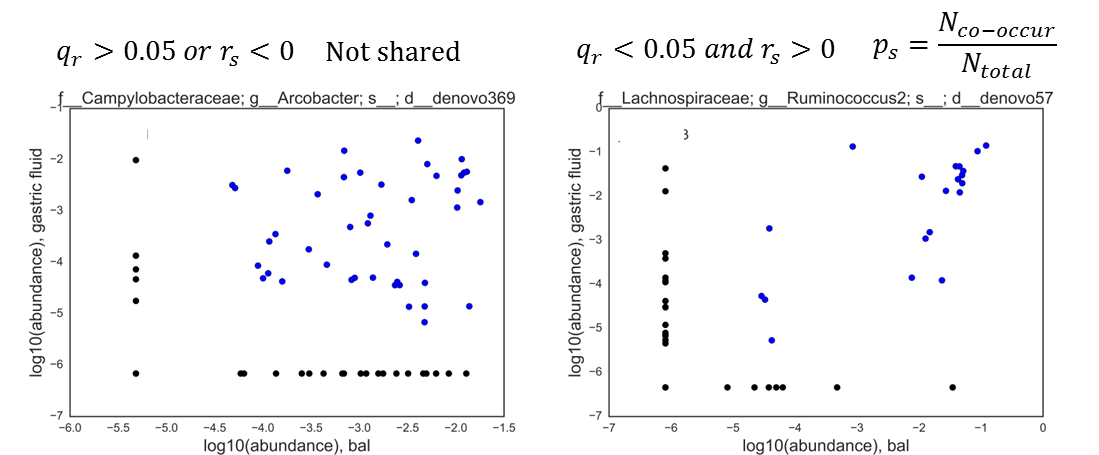
\includegraphics[scale=0.6]{sharedness_definition}
    \caption{Calculating $p_s$: if the abundance of a microbe when it is 
    present in both sites is correlated, then we consider it exchanged 
    across those sites (blue dots). $p_s$ is then calculated as the 
    percentage of patients who have the microbe present in both sites (blue 
    dots divided by total dots). Example of microbes which are (A) not 
    exchanged and (B) exchanged between stomach and lungs.}\label{fig:sharedness_defn}
\end{center}
\end{figure}
%\end{wrapfigure}

\subsubsection{Identify clinical modulators of lung, gastric, and throat microbial communities}
Once we quantify microbial exchange within the aerodigestive tract, we 
can begin to ask which clinical factors modulate the exchange 
occurs between sites. We hypothesize that aspiration will modulate the 
amount of throat-lung and gastric-lung exchange, that reflux will modulate 
the amount of gastric-lung exchange, and that PPI use may also affect
the gastric-lung connection, or may simply change the whole communities.
For each of these clinical factors, we will calculate a new $p_s$ for 
each previously-defined exchanged microbe, within each patient subgroup.
In other words, $p_s'$ is the percent of the patients in one subgroup
that have each exchanged microbe present in both of the sites.
We will also investigate the overall community similarity (i.e. beta diversity) 
between the two sites for each patient subgroup. Finally, we may pursue
more exploratory analyses like univariate comparisons of OTU abundances
in patients with and without each condition.


Our first hypothesis is that aspirators will have more exchange between their throat and lungs and between their stomachs and their lungs.
Aspirating patients are at higher risk for respiratory infections, which
may be a result of stomach or oral microbes successfully seeding the lungs
because the airway is no longer adequately protected.
Reflux surgery is often prescribed to aspirators with chronic infections,
as it is thought that the refluxate of these patients carries microbes which seed the lungs. Our dataset has 48 patients with abnormal MBS test results (Aspirators) and 63 patients with normal results.

Our next hypothesis is that patients with more severe GERD will have 
more exchange between the stomach and lung communities. Because we are 
interested in GERD that may modulate the stomach-lung connection by
actually reaching the top of the esophogaus, we will focus our analyses
on proximal, i.e. full-column, reflux. Our GERD data quantifies the
percent of reflux which is full-column, and does not provide a hard
cutoff above which reflux is considered ``severe''. Thus, another goal
of this work is to identify if such a threshold exists. We will examine
how exchange between and similarity of the lung ang gastric communities
changes as a function of this ``severity'' cutoff. If we find a cutoff
in which the amount of exchange in patients who are above the cutoff is 
significantly higher than in patients who are below the cutoff, then perhaps
this threshold could define the clinically-relevant amount of reflux that is
problematic.

Finally, we will investigate how PPIs modulate the exchange between
all three aerodigestive sites. PPIs reduce the acidity of the gastric
fluid, which may increase the bacterial load of the refluxate and
lead to more frequent colonization of the lungs \cite{rosen-bal_culture-2011}.
We hypothesize that patients on PPIs will have altered gastric fluid
microbial communities, and that the exchange between the lungs and
stomach may be increased. The dataset has 114 patients on PPIs and 85 patients not on PPIs.

An important consideration when interpreting these results is that
this work does not address the direction of microbial exchange between 
aerodigestive sites, nor does it directly link increased microbial 
exchange with adverse outcomes like respiratory infections.
We assume that most of the community is being seeded from the throat, 
but do not explicitly know the balance between immigration, elimination, and 
growth of microbes in each site \cite{bassis-source-2015}.
Follow up studies focusing on patients who develop respiratory 
infections or who frequently have GERD- or aspiration-associated 
respiratory infections should be undertaken to directly link the exchange
between communities with adverse clinical outcomes. 


\subsection{Aim 2: Meta-analysis of gut microbiome studies}\label{sec:aim2}
By combining results from existing gut microbiome case-control 
studies, we can move the field toward a consolidated understanding of 
consistent microbial markers of gut-related diseases. We hypothesize 
that certain bacteria will often be associated with disease, and that 
some of these bacteria will be associated with many different types of 
diseases while others will be unique to one or two conditions. 
Additionally, we hypothesize that microbial signatures  of health and 
disease will be more similar in similar diseases (i.e. in diabetes and 
obesity vs. in diabetes and autism).

\subsubsection{Compile and process gut microbiome datasets}
To perform a meta-analysis, we need to collect a 
comprehensive selection of 16S gut microbiome case-control studies. We 
will identify these studies through a targeted literature search.  See 
TABLE for exclusion and inclusion criteria for studies to be 
considered.

We will process these datasets using a standardized in-house pipeline 
developed by Thomas Gurry, a post-doc in the Alm lab. We will 
start with the rawest available data - in most cases, these will be 
fastq files but for some studies we will begin from quality-filtered 
fasta files. Sequences will be quality and length trimmed, clustered 
at 100\% similarity, and assigned Latin taxonomic names using the RDP 
classifier. Samples with fewer than 100 reads will be removed from 
consideration. OTUs with fewer than 10 reads or which are present in 
less than 1\% of samples will be removed. More stringent quality 
filtering may be considered in order to reduce noise in the dataset.

Because studies which sequence different 16S regions will have 
different sequences corresponding to the same bacteria, we can not 
used sequence-based open-reference approaches to compare OTUs across 
studies. After assigning Latin names based on OTUs within each study, 
we will collapse OTUs to the genus level and compare these across 
studies.

\subsubsection{Identify microbial markers of disease}\label{sec:indep_studies}
Once we have processed all datasets in a standardized way, our first 
goal is to identify microbial markers of general health and disease. 
For each study, we will compare macro-summaries of the microbial communities
(i.e. alpha diversity, Bacteroides/Firmicutes ratio) between cases and controls.
Then, we will look for specific microbes associated with health or disease using
univariate non-parametric statistics to compare abundances of microbes in cases
and controls. To identify microbes which are \textit{consistently} associated with
health or disease, we will combine the results from all studies using 
the weighted Z-test, a weighted method used in meta-analyses for combining p-values \cite{zavkin-ztest-2011}. 
This will yield an overall significance for each microbe,
incorporating the results from all case-control studies.

Next, we aim to identify microbes which are consistently associated with \textit{specific}
diseases. For diseases which have more than 3 studies, we will
perform the same meta-analysis as above with only the studies
of that disease. There are many interesting possible outcomes from this analysis.
First, we could find bacteria which are not associated with disease in general 
but which \textit{are} associated with that specific disease. 
We could also find bacteria which are significant markers of disease in general and 
that specific disease, but whose direction of change may differ in the two cases.
For example, a bacteria could be significantly higher in Parkinson's patients but
significantly lower in all other disease states. The microbes we identify with this
analysis may be very interesting candidates for biomarkers or mechanistic follow-up studies.

It is possible that we struggle to find bacteria consistently 
associated with diseases because of technical batch effects, even 
where we expect to find a clear signal (i.e. in diseases which have 
had clear results from experimental or mechanistic studies (REFS)). 
Developing robust methods to overcome technical batch effects in 16S 
studies is not within the scope of this work. However, if standard 
meta-analysis methods fail, we can try some naive linear correction methods 
like subtracting the components which correlate closely with technical 
artifacts like read depth (FIGURE?). We could 
also consider using a phylogenetics-based approach rather than 
taxonomically-assigned closed-reference OTUs. In other words, we could use open-referenced OTUs to identify 
associations with disease within each dataset and then compare 
the phylogenetic relationship of significant OTUs across all studies. Finally, we could 
approach our meta-analysis from a functional point of view by
using tools like PiCRUST or HUMANN to assign functionality to our
observed taxonomies \cite{langille-picrust-2013}, \cite{abubucker-humann-2012}.


\subsubsection{Compare results between studies for related diseases}\label{sec:signatures}
Our next hypothesis is that similar diseases will have similar 
signatures of dysbiosis. For example, we expect that metabolic 
diseases like obesity and diabetes will have more similar microbiota 
changes than they will to diarrheal diseases like \textit{Clostridium 
difficile} infection or enteric diarrhea. We will summarize each 
dataset with one vector indicating its "microbial signature". This 
signature will be based on number and identities of microbes 
significantly associated with the cases and the direction of change 
of these microbes relative to the controls. Depending on the results from Section 
\ref{sec:indep_studies}, we may also include factors like differences 
in alpha diversity or Bacteroides/Firmicutes ratios. Then, we will 
investigate which datasets cluster together in this "signature space". 
(Fig. \ref{fig:microbe_signatures})

%\begin{wrapfigure}{R}{0.5\textwidth}
%	\centering
\begin{figure}
\begin{center}
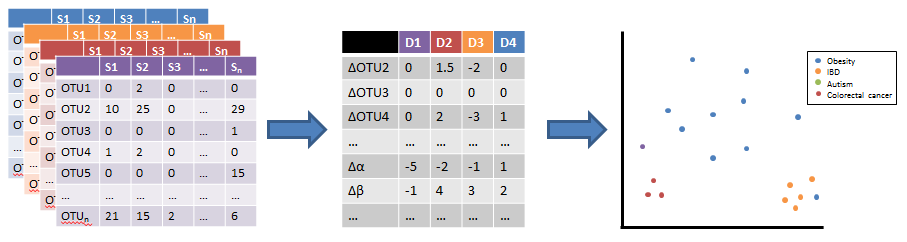
\includegraphics[scale=0.5]{microbial_signatures}
\caption{Defining microbial signatures}\label{fig:microbe_signatures}
\end{center}
\end{figure}
%    \caption{Defining microbial signatures}
%\label{fig:microbe_signatures}
%\end{wrapfigure}

If a disease has a strong impact on or association with the gut 
microbiome, then we would expect its signatures from multiple studies 
to cluster very tightly together. If this is the case, we can extract 
the bacterial features which contribute the most to this tight 
clustering - these will then be most likely to be associated with that 
specific disease, and would be good candidates for further mechanistic 
explorations. On the other hand, if datasets of the same disease or 
similar conditions do not have similar microbial signatures, this may 
indicate that the microbiome is not inherently implicated in or affected 
by the disease. In this case, any signal that we see in the gut 
microbiome is likely driven by other non-disease effects, which are 
not necessarily the same across studies. Finally, if we find different 
diseases with similar underlying causes (i.e. inflammation) clustering 
near each other, then perhaps this would indicate that the microbiome 
is affected or involved with the underlying cause rather than the 
specific diseases. Such insights could help us design better 
experiments to follow up on mechanism or causal relationships.

\subsection{Aim 3: Assigning bacteria to groups with similar functions and disease associations}

In this aim, we will curate biologically-motivated \textit{microbe 
sets} to enable easier interpretation of results from 16S microbiome 
analyses. By defining groups of related microbes \textit{a priori}, we 
will enable enrichment analyses similar to GSEA (\ref{sec:gsea}, 
\cite{subramanian-gsea-2005}) for microbiome data. Enrichment analyses will allow for better 
biological understanding of individual studies' results as well as 
more consistent comparisons of results across individual studies in 
the literature.

\subsubsection{Define microbe sets based on known biological relationships}

Our first task is to curate and define \textit{microbe sets} for use in enrichment analyses of 
microbiome datasets. We will perform an extensive literature search
to identify existing databases and review papers with validated microbial phenotype annotations, with the goal of
combining these databases and filling them out where they are missing annotations.
We will begin with ImG which has approximately 10,000 annotated microbial genomes. 
About half of these genomes are human-associated bacteria, 
and half of those have annotations for categories like disease 
association, sporulation, and body site habitat. 
We will extract the 16S sequences for all the annotated human-associated 
microbes in this dataset, build a phylogenetic tree, and determine whether 
they adequately span the phylogenetic diversity we expect to 
find in the human gut. If certain key clades are missing from these 
bacteria, we will manually include them from literature searches and 
NCBI queries.

In collaboration with Ilana Brito at Cornell, we will apply a 
combination of literature mining and bioinformatics approaches to fill 
out the missing annotations in the databases and to add our own fields 
of interest \ref{tab:microbe_set_categories}. We may also 
pursue unsupervised text mining of literature results to infer trait-
associations for well-studied bacteria \cite{korbel-lit_mining-2005}. As we populate 
our microbe annotations, we will also collect the relevant 16S sequences to 
build a tree. When possible, we apply appropriate inference models to infer 
missing traits of leaf organisms when possible.

\begin{table}
\begin{tabular}{|p{6cm}|p{10cm}|}
	\hline
	\textbf{Category} & \textbf{Approach} \\
	\hline
	Pathogens & Targeted literature search, literature mining, \& 
	databases \\
	\hline
	Body sites & Literature mining, machine learning on HMP data \\
	\hline
	Environmental associations & Literature mining, machine learning 
	on EMP data \\
	\hline
	Growth rate & Inference from 16S sequences in datasets from Aim 2 
	and HMP \\
	\hline
	Obesity-associated & Targeted literature search \& machine 
	learning on Aim 2 datasets \\
	\hline
	Inflammation-associated & Targeted literature search \& machine 
	learning on Aim 2 datasets \\
	\hline
	Miscellaneous functions (acid-tolerant, mucus-degrading, etc) & 
	Targeted literature search, unsupervised PiCRUST clustering, 
	genome mining \\
	\hline 
\end{tabular}
\caption{Possible approaches to define microbe sets of interest}\label{tab:microbe_set_categories}
%\end{wraptable}
\end{table}


\subsubsection{Extract disease-associated microbe sets from datasets in Aim 2}
We will leverage the datasets collected in Aim 2 to extract additional 
disease-associated groups of microbes. We will define groups of 
microbes based on those that distinguished diseases or broader 
phenotypes in Section \ref{sec:signatures}. We will also pursue 
machine-learning driven approaches to identify novel disease- or 
phenotype-associated \textit{microbe sets}. We will define 
\textit{microbe sets} based on the most discriminating features of 
various comparisons, as described in Table \ref{tab:classifications}.

\begin{table}
\begin{center}
\begin{tabular}{|p{6cm}|p{10cm}|}
	\hline
	\textbf{Microbe set association} & \textbf{Classification task} \\
	\hline
	General health/disease & All healthy vs. all disease \\
	\hline
	Diarrhea & CDI, EDD, IBS-D vs. controls \\
	\hline
	Neurological & Autism, Parkinson's vs. controls \\
	\hline
	Immune system & Rheumatoid arthritis, allergy, Crohn's disease, 
	Graft-versus-host disease vs. controls \\
	\hline
	Liver & NASH, MHE (all hepatic diseases) vs. controls\\
	\hline
	Metabolic syndrome & T1D, T2D, obesity, metabolic syndrome vs. 
	controls \\
	\hline
\end{tabular}
\caption{Classification tasks to identify groups of phenotype-
associated microbes}\label{tab:classifications}
\end{center}
\end{table}

\subsubsection{Develop collaborative tool for interpreting microbiome studies}
We will make the microbe set annotations available to researchers for 
further annotation and development. Through our literature searches, 
we will pay attention to the databases researchers have found most 
useful and strive to package our annotations in an easy-to-use format. 
We will likely begin with one very large text file containing all of 
the microbes, 16S sequences, and metadata that we have gathered. 

We will also package our \textit{microbe set} annotations into a tool 
that researchers can use to interpret the results of their 16S 
studies. Our software will take as input an OTU table with 
taxonomically assigned microbes and disease-state labels for samples. 
It will perform enrichment analysis on the OTU table and return the 
results to researchers, similar to the Broad's GSEA tool \cite{subramanian-gsea-2005}. All of this work will be done using public open-source tools like 
GitHub to encourage collaboration and dissemination of our findings.

Developing a database of microbial annotations is a daunting task due 
to the vast diversity and complexity of microbes. We recognize the 
inherent difficulty of this task, and do not expect to produce a fully 
comprehensive database. However, because our annotations are intended 
to serve as a tool for biological interpretations and hypothesis 
generation, even a partially-complete database will be extremely 
valuable in reducing the number of false-negative results in case-
control studies and also providing coherent biological interpretations 
of existing results. We also recognize that our work will be just the 
beginning of systematic grouping of phenotypically-associated 
microbes, and so we will ensure that the format of the database we 
develop is easily accessible and modifiable by other researchers.

This work will be the beginning of what will hopefully become a new 
approach to interpreting 16S datasets - moving the field from asking 
simply ``what's different?'' toward a more critical interpretation of 
``why are things different?''

\section{Preliminary studies}
\textit{Three to four pages}

\subsection{Aim 1}
\subsubsection{Microbiome community exchange}
Using our definition of $p_s$ (\ref{sec:exchange}), we identified over 100
OTUs exchanged across sites of the aerodigestive tract.
As expected, the majority of these were exchanged between the throat and stomach.
Interestingly, the stomach and lungs also had a significant
amount of microbial exchange, and these communities were almost as similar to
each other as the throat and stomach communities were. 
These findings support the hypothesis that frequent microaspiration
of gastric contents into the lungs is occurring. While certain bacteria
may be preferentially exchanged between the lungs and stomach, the lower 
number of exchanged microbes as compared to the throat and lungs, combined with
the similar similarity of communities, indicates that much of the exchange may
be more stochastic, and not selecting for specific community members
across many patients.
Finally, we observed a decreasing trend in number of exchange microbes 
across throat-stomach, lung-stomach, and throat-lung sites, respectively, 
for all phyla except Proteobacteria. More Proteobacteria were exchanged 
between lungs and stomach than throat and stomach. Proteobacteria are 
known aerobes, and so may be preferentially selected for colonization in 
the lungs after microaspiration from the stomach.

\subsubsection{Modulators of community exchange}
We observed a distinct difference in the amount of exchange between the 
throat and lungs of aspirators versus patients with normal MBS results.
We looked at the previously-defined microbes that were exchanged between 
the throat and lungs and re-caculated $p_s$, the percent of patients
who have that microbe present in both sites, for the aspirator and 
non-aspirator groups separately. 25\% of aspirators shared
these microbes across their throats and lungs, while only 13\% of 
non-aspirators did. Additionally, the throat and lung communities
were significantly more similar in aspirating patients than non-aspirators. These results indicate that a consequence of abnormal swallowing
dysfunction is likely a seeding of the lungs with oral bacteria.
Interestingly, the stomach and lung communities of aspirating
patients were slightly more similar to each other than in non-aspirators.
By definition, aspirating patients are unable to protect their airways
from foreign material - while most apparent in swallowing, such dysfunction
may also enable more material to move between the stomach and lungs as well.

The effect of reflux on the stomach-lung connection was less striking 
but still apparent. Specifically, the stomach and lung communities were
more similar to each other in patients with very frequent full-column reflux. However, here was no significant difference in the extent of
microbial exchange between the stomach and lungs. In other words,
the previously-defined stomach-lung exchanged microbes were as likely
to be found in both sites in patients with frequent full-column reflux
than in patients with less severe reflux. This may indicate a more
stochastic seeding of the lungs from the stomach rather than reproducible
exchange of the same microbes across patients. In this case, stomach 
microbes are not necessarily growing in the lungs but nonetheless do have 
measurable impact on the lung's microbial community.

\subsection{Aim 2}
\subsubsection{Collecting and reprocessing 16S case-control datasets}
Our extensive literature review has so far identified 54 suitable case-control 16S datasets.
29 datasets and their associated metadata have been downloaded and processed through our in-house pipeline.
Characteristics of these datasets are shown in Table \ref{tab:datasets}

\begin{table}
\begin{tabular}{|c|c|c|c|c|c|}
	\hline
	\textbf{Dataset ID} & \textbf{Diseases} & \textbf{Median reads/sample} & \textbf{Year} & \textbf{Platform} & \textbf{Region} \\
	\hline 
\end{tabular}
\caption{Datasets}\label{tab:datasets}
\end{table}

\subsubsection{Identify general patterns of health and diseases}
We first summarized overall community structure using Shannon's alpha diversity
index (SDI). We observed significant batch effects across studies, likely due to
the differences in sequencing depth. After standardizing SDI within studies
and combining similar disease states, we observed little difference in overall
community structure between cases and controls. An exception to this was seen
in diarrheal diseases (\textit{Clostridium difficile} infection and enteric 
diarrheal disease), in which alpha diversity was significantly lower in the cases. 

We next performed univariate comparisons at the genus level for abundance in cases 
vs. controls for each study. This analysis revealed a similar result: diarrheal 
diseases showed striking shifts in many microbes, while other
diseases had less obvious patterns of dysbiosis. We observed that many bacteria
seemed to have relatively consistent shifts between cases and controls across many
different diseases \ref{fig:pval_heatmap}. This supports the hypothesis that
there is a general signature for disease, in other words, that sick people have 
altered microbiomes. In light of this finding, identifying microbial shifts that 
are unique to individual diseases will be crucial to finding specific biomarkers
for diagnostic purposes and to motivate mechanistic investigations.

\section{Gud werds}
We hypothesize that there is a clinically-relevant exchange of bacteria within the aerodigestive tract that may be altered in certain disease states. 


Another important consideration in this work may be if study-associated effects are larger than biological effects. For example, when we compare 'microbial signatures' across datasets, it's possible that the largest signal driving dataset clustering is sequencer or 16S region sequenced, rather than disease state. There are many approaches we could take to correct for such batch effects:
\begin{enumerate}
	\item Subtracting the principal components corresponding to the technical artifacts.
	\item Build a model that accounts for these technical artifacts by including them as factors in the model.
	\item Non-parametric correction, like sample- or OTU-wise quantile normalization, using controls in each study as the reference distribution.
\end{enumerate}

This work will improve our 
understanding of the clinical relevance of the human microbiome and 
will also provide new approaches and tools for analyzing future 
studies.

We will summarize each dataset's microbial communities
methods commonly used in the 
literature: univariate non-parameteric statistical tests on relative 
abundances, alpha and beta diversity in different types of patients, 
and ratios of Firmicutes to Bacteroides in healthy vs. disease 
patients. It is generally thought that low alpha diversity is a marker 
of dysbiosis (REF), and that while most people have a Firmicutes/
Bacteroides ratio of (XXX), in certain diseases this ratio may be 
different (REF). (MAYBE BACKGROUND?) By analyzing each study in the 
same way from raw data, we can reduce the study-wise batch effects and 
increase our ability to identify general trends in the gut microbiome 
in health and disease. We will identify consistent markers of disease 
by using standard meta-analysis methods, comparing the effect sizes 
and directionality of bacteria across studies, and using Fisher's 
method to determine overall significant of a microbe (REFS). 

"Thus, humans are super organisms: http://science.sciencemag.org/content/312/5778/1355"

The microbiota of 
the aerodigestive tract is poorly studied, and we have little understanding 
of how the microbial communities in different aeordigest sites are related or 
affected by disease. In contrast, the gut microbiome has 
been extensively studied through many case-control studies. 
However, these studies have frequently yielded inconsistent or incomparable 
results. Existing meta-analyses have not extended to more than one or two 
diseases, and thus can not determine whether significant microbes are 
associated with specific diseases or with disease in general. 
Finally, there are no existing tools that can be used to extract general 
biological insights from groups of disease-associated microbes.

Fecal microbiota transplants have demonstrated the incredible
causal ability of the microbiome to affect health in 
human patients. Germ-free mouse models have shown that microbes are
necessary for healthy functioning, and specific animal models have  
allowed for probing mechanistic understanding of host-microbial 
interactions (autism 440 ref, gordon mouse experiment ref). 

Additionally, many of the most successful existing meta-analyses 
combine vastly different types of microbial communities and non-case-
control experimental designs. The positive results from these studies 
are not particularly biologically insightful: it is a much easier task 
to differentiate vastly different communities (like the skin vs. the 
gut) than it is to differentiate subtleties contributing to health and 
disease (like the inflamed gut vs. the healthy gut) \cite{knights-supervised-2010}.

Every meta-analysis performed on 16S data has observed 
strong batch effects between studies and noted the need for large 
sample sizes to extract any meaningful signal \cite{sze-signal-2016},
\cite{walters-ob_meta-2014},\cite{knights-supervised-2010},
\cite{lozupone-meta-2013}. 

This definition depends on correlated abundances and not simply co-occurence, and is 
superior to simple co-occurence because of the significant overlap in the
members of the three aeordigestive communities\cite{bassis-source-2015}, \cite{charslon-topographical-2011}.

To determine how lung, gastric, and throat microbial communities are related,
we will calculate $p_s$ for each of the site combinations. We will 
then see if there are apparent phylogenetic relationships between
the exchanged microbes. We expect to find significantly more exchange
between the throat and stomach, and very little exchange between the throat and lungs. 


\bibliographystyle{unsrtnat}
\bibliography{refs}

\end{document}